\documentclass{awesomecv}

\usepackage{geometry}
\geometry{
  left  =  30mm,
  right =  30mm,
  bottom = 40mm,
  top =    40mm
}

\documentcolor{blue}
\secondcolor{base01}
\thirdcolor{base01}
\sectioncolor{base02}

\titlethicknessleft{3mm}

\voiceleftsize{2.1cm}
\voicerightsize{12cm}

\begin{document}

\begin{titlebox}
  \authorname{Raoul Wols}{\emph{curriculum vit\ae}}

  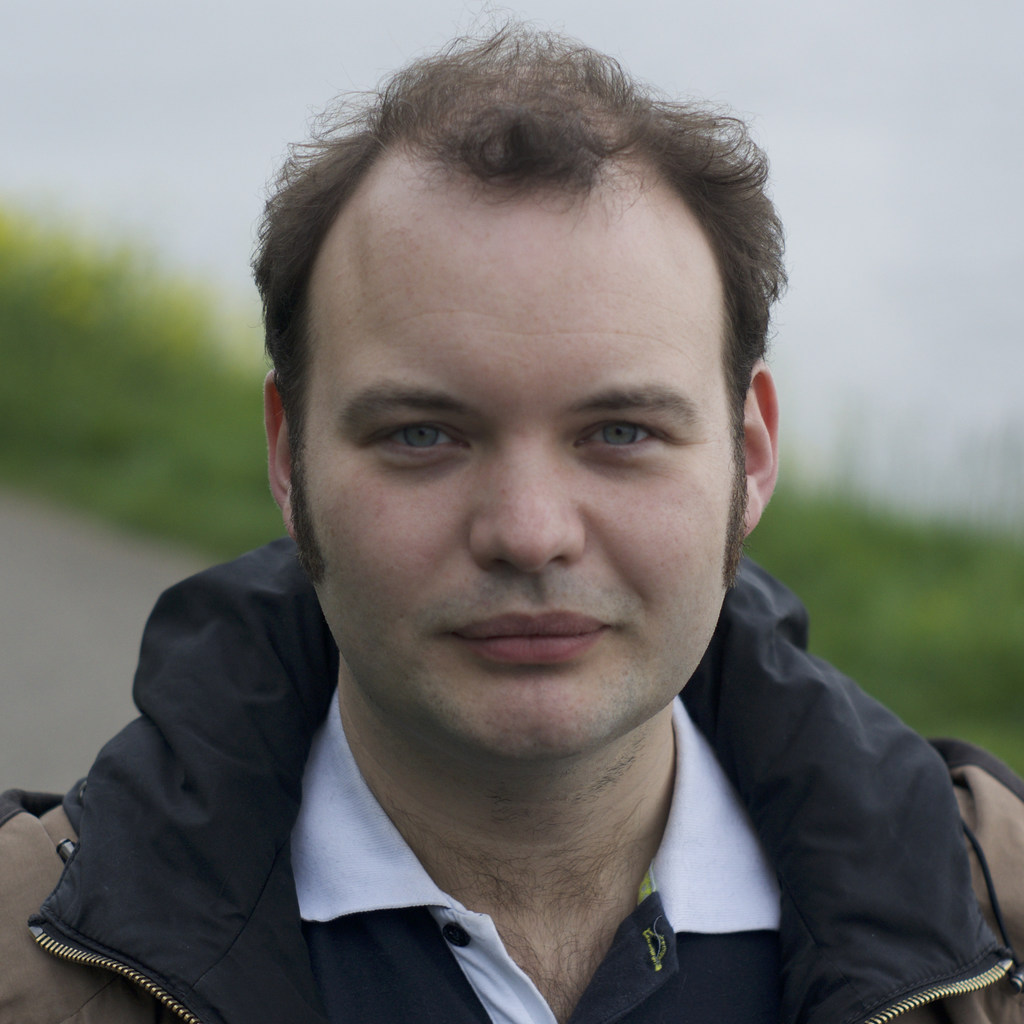
\includegraphics[scale=.2]{pics/me.jpg}
  % \qrcode{pics/qrcode.png}

  \tcblower

  \begin{showinfo}
    \birthdate{January 19th, 1989}
    \location{Slobbengorsweg 129}
    \location{3351LH Papendrecht}
    \location{The Netherlands}
    \mobile{+31 (0) 6 10917383}
    \firstMail{raoulwols@gmail.com}
    \firstMail{r@primef.actor}
    \github{https://github.com/rwols}
    \stackoverflow{stackoverflow.com/users/990142}
    \twitter{https://twitter.com/rwols}
  \end{showinfo}

\end{titlebox}

\updated{\today}

\opensection{\faGraduationCap}{Education}
\begin{describesection}

  \leftside{from \textbf{sep 2001} to \textbf{june 2007}}
  \rightsidecomplex{Gymnasium}{Johan de Witt Gymnasium}{Dordrecht, The Netherlands}{\;}

  \leftside{from \textbf{sep 2007} to \textbf{june 2010}}
  \rightsidecomplex{Minor Jazz Piano}{Royal Conservatory of The Hague}{The Hague, The Netherlands}{Final grade: 7.5}

  \leftside{from \textbf{sep 2007} to \textbf{july 2012}}
  \rightsidecomplex{Bachelor of Science in Mathematics}{Leiden University}{Leiden, The Netherlands}{Final grade: 7}

  \leftside{thesis}
  \rightsideplain{\textsc{Eindige Topologische Ruimten}}
  \leftside{advisor}
  \rightsideplain{Dr. R.S. de Jong}

  \leftside{\bf from sep 2012 to july 2016}
  \rightsidecomplex{Master of Science in Mathematics}{Leiden University}{Leiden, The Netherlands}{Final grade: 7.5}

  \leftside{thesis}
  \rightsideplain{\textsc{A McCord Functor for Alexandroff Categories}}
  \leftside{advisor}
  \rightsideplain{Dr. O.D. Biesel}

\newpage
\end{describesection}
\opensection{\faFire}{Extracurricular Activities}
\begin{describesection}
    \leftside{from \textbf{sep 2007} to \textbf{sep 2008}}
    \rightsidecomplex{Treasurer of Music Committee}{De Leidsche Flesch}{Leiden, The Netherlands}{I was treasurer of a newly-founded committee that would encourage and incentivize students in the exact sciences faculty to get on stage and show their artistic talents.}
    \leftside{from \textbf{sep 2008} to \textbf{sep 2009}}
    \rightsidecomplex{Chairman of Music Committee}{De Leidsche Flesch}{Leiden, The Netherlands}{The next year I became chairman of the same committee. The committee is still going strong as of this writing.}
    \leftside{from \textbf{sep 2007} to \textbf{sep 2014}}
    \rightsidecomplex{Keyboardist}{``The Circumstances''}{The Netherlands}{I played keyboards in an indie-rock band. We played at lots of places like The Melkweg in Amsterdam, 013 in Tilburg. We made an album that's available on iTunes.}
    \leftside{from \textbf{sep}}
    \rightsidecomplex{Baritone}{Barbershop quartet ``Auto o' Tune''}{The Hague area}{I sang baritone in a quartet.}
\end{describesection}

\opensection{\faFlask}{Experience}
\begin{describesection}

  \leftside{from \textbf{july 2011} to \textbf{jan 2012}}
  \rightsidecomplex{Intern}{RoserConSys B.V.}{Dordrecht, The Netherlands}{I researched resource constrained project scheduling problems. i.e. finding algorithms that will produce, in polynomial time, a "good" schedule. A resource constrained project scheduling problem is of class NP-hard if the goal is to find the optimal schedule. The languages were VB.NET and C++.}

  \leftside{from \textbf{sep 2008} to \textbf{jan 2009}}
  \rightsidecomplex{Tutor}{Leiden University Math Faculty}{Leiden, The Netherlands}{I assisted a small group of students with their homework.}

  \leftside{from \textbf{jan 2013} to \textbf{july 2014}}
  \rightsidecomplex{Teaching Assistant}{Leiden University Math Faculty}{Leiden, The Netherlands}{I assisted students in the Algebra 1 course.}

  \leftside{from \textbf{july 2016} to \textbf{jan 2017}}
  \rightsidecomplex{Founder}{Primef.actor Entertainment}{Papendrecht, The Netherlands}{I dedicated my time to create a video game called
  "Alien Invasion Game". The engine used was Unity, so everything is written in C\#.}
\end{describesection}

\newpage
\opensection{\faCogs}{Projects}
\begin{describesection}

  \leftside{name}
  \rightsideplain{\color{blue}Plan-IT}
  \leftside{language}
  \rightsideplain{\emph{VB.NET}}
  \leftside{description}
  \rightsideplain{Scheduling software with a GUI for which I wrote a proof-of-concept genetic algorithm.}

  \\

  \leftside{name}
  \rightsideplain{\color{blue}Firing Neurons}
  \leftside{type}
  \rightsideplain{\emph{EP}}
  \leftside{description}
  \rightsideplain{An Indie-Rock EP released on iTunes. I played keyboards.}

  \\

  \leftside{name}
  \rightsideplain{\color{blue}gintonic}
  \leftside{language}
  \rightsideplain{\emph{C++}}
  \leftside{description}
  \rightsideplain{A hobby render engine. The current render method is deferred.}

  \\

  \leftside{name}
  \rightsideplain{\color{blue}Alien Invasion Game}
  \leftside{language}
  \rightsideplain{\emph{C\#}}
  \leftside{description}
  \rightsideplain{A 2D platformer with shoot mechanics. Can be found at rwols.itch.io.}

  \\

  \leftside{name}
  \rightsideplain{\color{blue}Clara}
  \leftside{language}
  \rightsideplain{\emph{C++ and Python}}
  \leftside{description}
  \rightsideplain{Sublime Text 3 plugin for semantic C++ auto-completions. This has a compiled component. So the main language is C++, with some Python bindings.}

  \\

  \leftside{name}
  \rightsideplain{\color{blue}yaml-archive}
  \leftside{language}
  \rightsideplain{\emph{C++}}
  \leftside{description}
  \rightsideplain{A drop-in replacement for boost::archive::xml\_oarchive and boost::archive::xml\_iarchive
  from the Boost.Serialization library.}

  \\

  \leftside{name}
  \rightsideplain{\color{blue}CMakeBuilder}
  \leftside{language}
  \rightsideplain{\emph{Python}}
  \leftside{description}
  \rightsideplain{Sublime Text 3 plugin for building CMake projects.}

\end{describesection}

\newpage
\opensection{\faComments}{Natural Languages}
\begin{describesection}

  \leftside{\color{blue}Dutch}
  \rightsideplain{Mother tongue.}

  \leftside{\color{blue}English}
  \rightsideplain{Fluent in conversation and comprehension.}

  \leftside{\color{blue}German}
  \rightsideplain{Basic knowledge.}

  \leftside{\color{blue}French}
  \rightsideplain{Basic knowledge.}

\end{describesection}

\opensection{\faComments}{Programming Languages}
\begin{describesection}

  \leftside{\color{blue}C++}
  \rightsideplain{Expert in language and standard library usage.}

  \leftside{\color{blue}C\#}
  \rightsideplain{Expert in language, adequate in standard library usage.}

  \leftside{\color{blue}Python}
  \rightsideplain{Adequate in language and standard library usage.}

  \leftside{\color{blue}TeX}
  \rightsideplain{Expert in (markup) language.}

  \leftside{\color{blue}HTML, CSS}
  \rightsideplain{Average experience.}

  \leftside{\color{blue}GLSL}
  \rightsideplain{Very good experience in language and library usage.}

  \leftside{\color{blue}HLSL}
  \rightsideplain{Some experience; mainly via Unity. It's basically the same as GLSL.}

  \leftside{\color{blue}CMake}
  \rightsideplain{Expert in language and library.}

  \leftside{\color{blue}JavaScript}
  \rightsideplain{Some experience; but it's prototyped and dynamic like Python, so easily learned.}
\end{describesection}

\opensection{\faComments}{Programming Miscellaneous}
\begin{describesection}
\leftside{Methodologies}
\rightsideplain{agile, waterfall.}
\leftside{Design Patterns}
\rightsideplain{object-oriented, functional, data-driven, factory, abstract factory, lazy initialization, singleton (but don't ever use this!), RAII, facade, flyweight,  command pattern, iterator, the none object, the visitor, thread pool, locking and joining, consumer-producer, strategy pattern, loose coupling,
curiously recurring template pattern, substitution-failure-is-not-an-error.}
\leftside{Tools Experience}
\rightsideplain{Visual Studio, Xcode, Sublime Text (my favourite right now), clang, clang-cl, gcc, cl, msbuild, ninja, cmake, gdb, lldb.}
\end{describesection}

\end{document}
